\subsection*{b)}
In this assignment we will provide a parametric bootstrapped 95\% confidence interval for the parameters. Since we have a dataset that we can evaluate parameters from, we need to determine the uncertainty of the estimators. To assess the uncertainty we analyze the distribution function $F_{\Delta}$ of the error $\Delta$ under $\mathbb{P}_0$. This uncertainty can be bounded by confidence intervals to assess the uncertainty we analyze the distribution function $F_{\Delta}$ of the error $\Delta$ under $\mathbb{P}_0$. \\

First of, we begin the bootstrap as described previously. We therefore estimate the parameters of the data by the function \texttt{est\_gumpel.m}. These estimates are the frequentistic approach using maximum likelihood. We then sample new data by generating random numbers and sampling using the inverse method of the relation derived in section \textbf{a)}. Thereafter we calculate the error of our estimates by the relation $\Delta_b^*(t)=\hat{t}_b^*-\hat{t}$. To get the confidence bounds for our estimates we used the relation \eqref{conf} derived in Jimmy Olssons lecture notes \cite{JO} 
\begin{equation} I_{\alpha}=\left(t(y) - F_\Delta^{-1}(F_\Delta^{-1}(1-\alpha/2),t(y)-F_\Delta^{-1}(\alpha/2)\right).
\label{conf}
 \end{equation}

However, we also need to check the bias of our estimate by the relation
\[ B_t=\mathbb{E}_0(t(Y)-\tau)=\mathbb{E}_0(\Delta(Y))=\int zf_\Delta (z) dz, \]
where $f_\Delta(z)=\frac{d}{dz}F_\Delta(z)$ denoting the density of $\Delta(Y)$. The calculated bias of the estimator for $\mu$ and $\beta$ respectively was computed as 
\[ B_t = \mathbb{E}_0(\Delta_b^*(t))=\left\{ \begin{array}{l}
-0.0009 \\ 0.0037
\end{array}\right. \]

The bias was then taken into consideration by making the bias-corrected estimate $t-B_t$. 

\begin{table}
\centering
\begin{tabular}{|c|c|c|}
\hline

 & L & U \\ \hline
%Estimates & 1.4858 & 4.1477 \\ \hline
$\beta$ & 1.3942 & 1.5821 \\ \hline
$\mu$ & 4.0220 & 4.2723 \\ \hline

\end{tabular}
\caption{Table showing the expected values and upper and lower bounds.}
\end{table}

In figure \ref{fig:estwaves} the histogram of the estimated dataset as well as the dataset is plotted.

\begin{figure}[H]
\centering
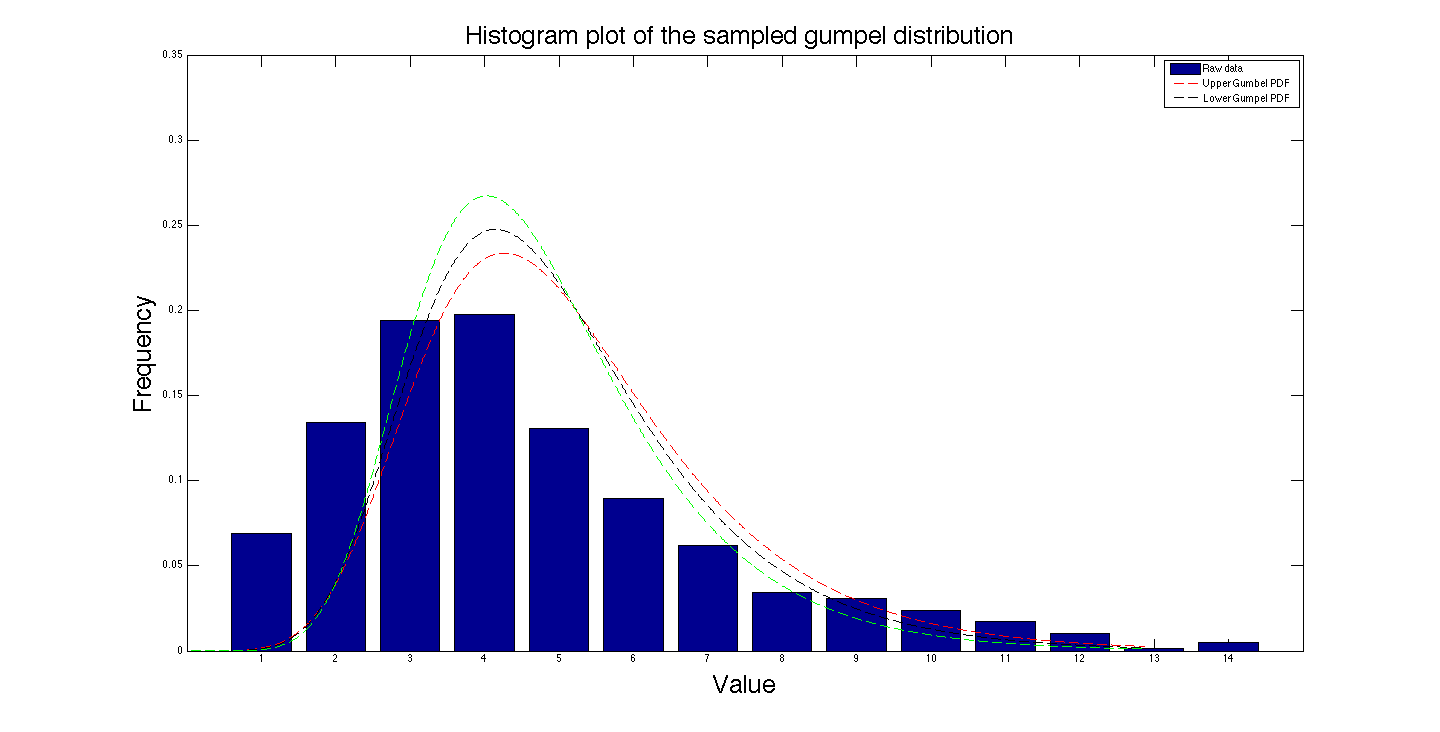
\includegraphics[scale=0.26]{./Figures/estwaves.png}

\label{fig:estwaves}
\caption{A histrogram of the estimated dataset, plotted over the real dataset.}
\end{figure} 

Here we can see the upper and lower cconfidence bound of the estimated wavesplotted with the raw data. One can observe that the gumpel approximation is indeed an approximation of the data.
